\subsection{Large Hadron Colllider}
% brochure: http://cds.cern.ch/record/1165534/files/CERN-Brochure-2009-003-Eng.pdf
% brochure, page 12-13 (16-17 of pdf doc)
Large Hadron Collider (LHC)~\cite{ref_LHC_brochure},~\cite{ref_LHC_TDR},~\cite{ref_LHC_website} is the last element of the chain of the CERN's accelerator complex (Fig.~\ref{fig:CERN_accelerator_complex}). Before entering LHC, particle beams are going through several stages of the acceleration. Thus, protons are extracted from hydrogen atoms, are accelerated by Linac2 to energies of~5~MeV, then injected into the Proton Synchrotron Booster (PSB) where they reach energies of~1.4~GeV. After that protons are to PS and Super PS (SPS) where they are accelerated to~25~GeV and~450~GeV respectively. Finally, protons enter LHC and are accelerated for 20 minutes to reach their design energies of~7~TeV per beam. \\

Besides protons, the complex also works with lead ions however in this dissertation we analyze data from proton-proton collisions only and, therefore, are not discussion lead ion collisions in more details.\\    

% brochure, page 15-17 - skip (19 of pdf doc)
% PLACE this sentence somewhere else; the rest of material is too basic

%brochure, page 18 (20 of pdf doc)
LHC is the largest particle accelerator ever built: it is about~27 km in circumference. Also LHC re-uses the tunnel built for Large Electron-Positron (LEP) Collider which determines the size of the machine. The large size is necessary to reach design high energies. \\

%brochure p 38 (42 of pdf doc) 
Main goals of LHC were to detect the Higgs boson if it existed and to search for evidences of BSM physics which may give a clue on understanding the phenomena which are not described by the SM including dark matter, matter-antimatter asymmetry, gravitational force and others. Six detectors are installed at the LHC to detect particles and perform the relevant measurements. There are general purpose detectors ATLAS and CMS, there is LHCb which specializes of the physics of B-mesons, ALICE which is designed to detect products of heavy ion collisions. In addition, there are two small detectros with very specific tasks: LHCf and TOTEM which are installed close to the ATLAS and CMS interaction points respectively. \\

No deviations from the SM were found by any of the experiments. The main achivement of the LHC to date is the discovery of the Higgs boson in 2012 by CMS \cite{ref_HiggsPaperCMS} and ATLAS \cite{ref_HiggsPaperATLAS} collaborations.\\

%brochure 27 (31 of pdf doc)

LHC is constructed of eight arcs, each arc corresponds to a sector as shown in Fig.~\ref{fig:LHCsectors}. In between there are eight insertions where beams are either collided or injected or dumped or cleaned.\\

From the other hand, LHC is split on eight octants, each starting from the middle of one sector and ending at the middle of the next one. Thus, each octant includes one full insertion.\\ 

Main parameters are summarized in Tab. \ref{tab:LHCparameters}.

Besides a beam energy, the most important quality of the accelerator is ability to produce a large number of interesting collisions which is determined by luminosity. The instantaneous luminosity is determined by the following expression \cite{ref_PDG}:\\

$L = f \frac{n_1 n_2}{4 \pi \sigma_x \sigma_y}$

where $n_1$ and $n_2$ are numbers of particles in colliding bunches, $f$ is a frequency of collisions, $\sigma_x$ and $\sigma_y$ are beam sizes in horizontal and vertical directions. \\

To determine the integrated luminosity, one has to integrate the instantaneous luminosity over time:\\

$L_{int}=\int L dt$\\

Run periods of LHC in 2010-2012 refer to Run~I of the LHC operation. While working on energy of $\sqrt{s}=7$~TeV (3.5~TeV pae beam), LHC delivered~44.96~pb$^{-1}$ and~6.1~fb$^{-1}$ of data in 2010 and 2011 year respectively. In~2012 the working energy of LHC was $\sqrt{s}=8$~TeV, and the integrated luminosity was $L_{int}=$23.3~fb$^{-1}$.  After a long shutdown, LHC was upgraded for Run~II, to operate on $\sqrt{s}=13$~TeV in 2015 and delivered 4.22~fb$^-1$ of data by the end of 2015. In 2016 LHC continues operation on $\sqrt{s}=13$~TeV and by the end of September the integrated luminosity already exceeded a value of 30~fb$^{-1}$ \cite{ref_LHClumi_twiki}.\\ 

\begin{figure}[htb]
  \begin{center}
    {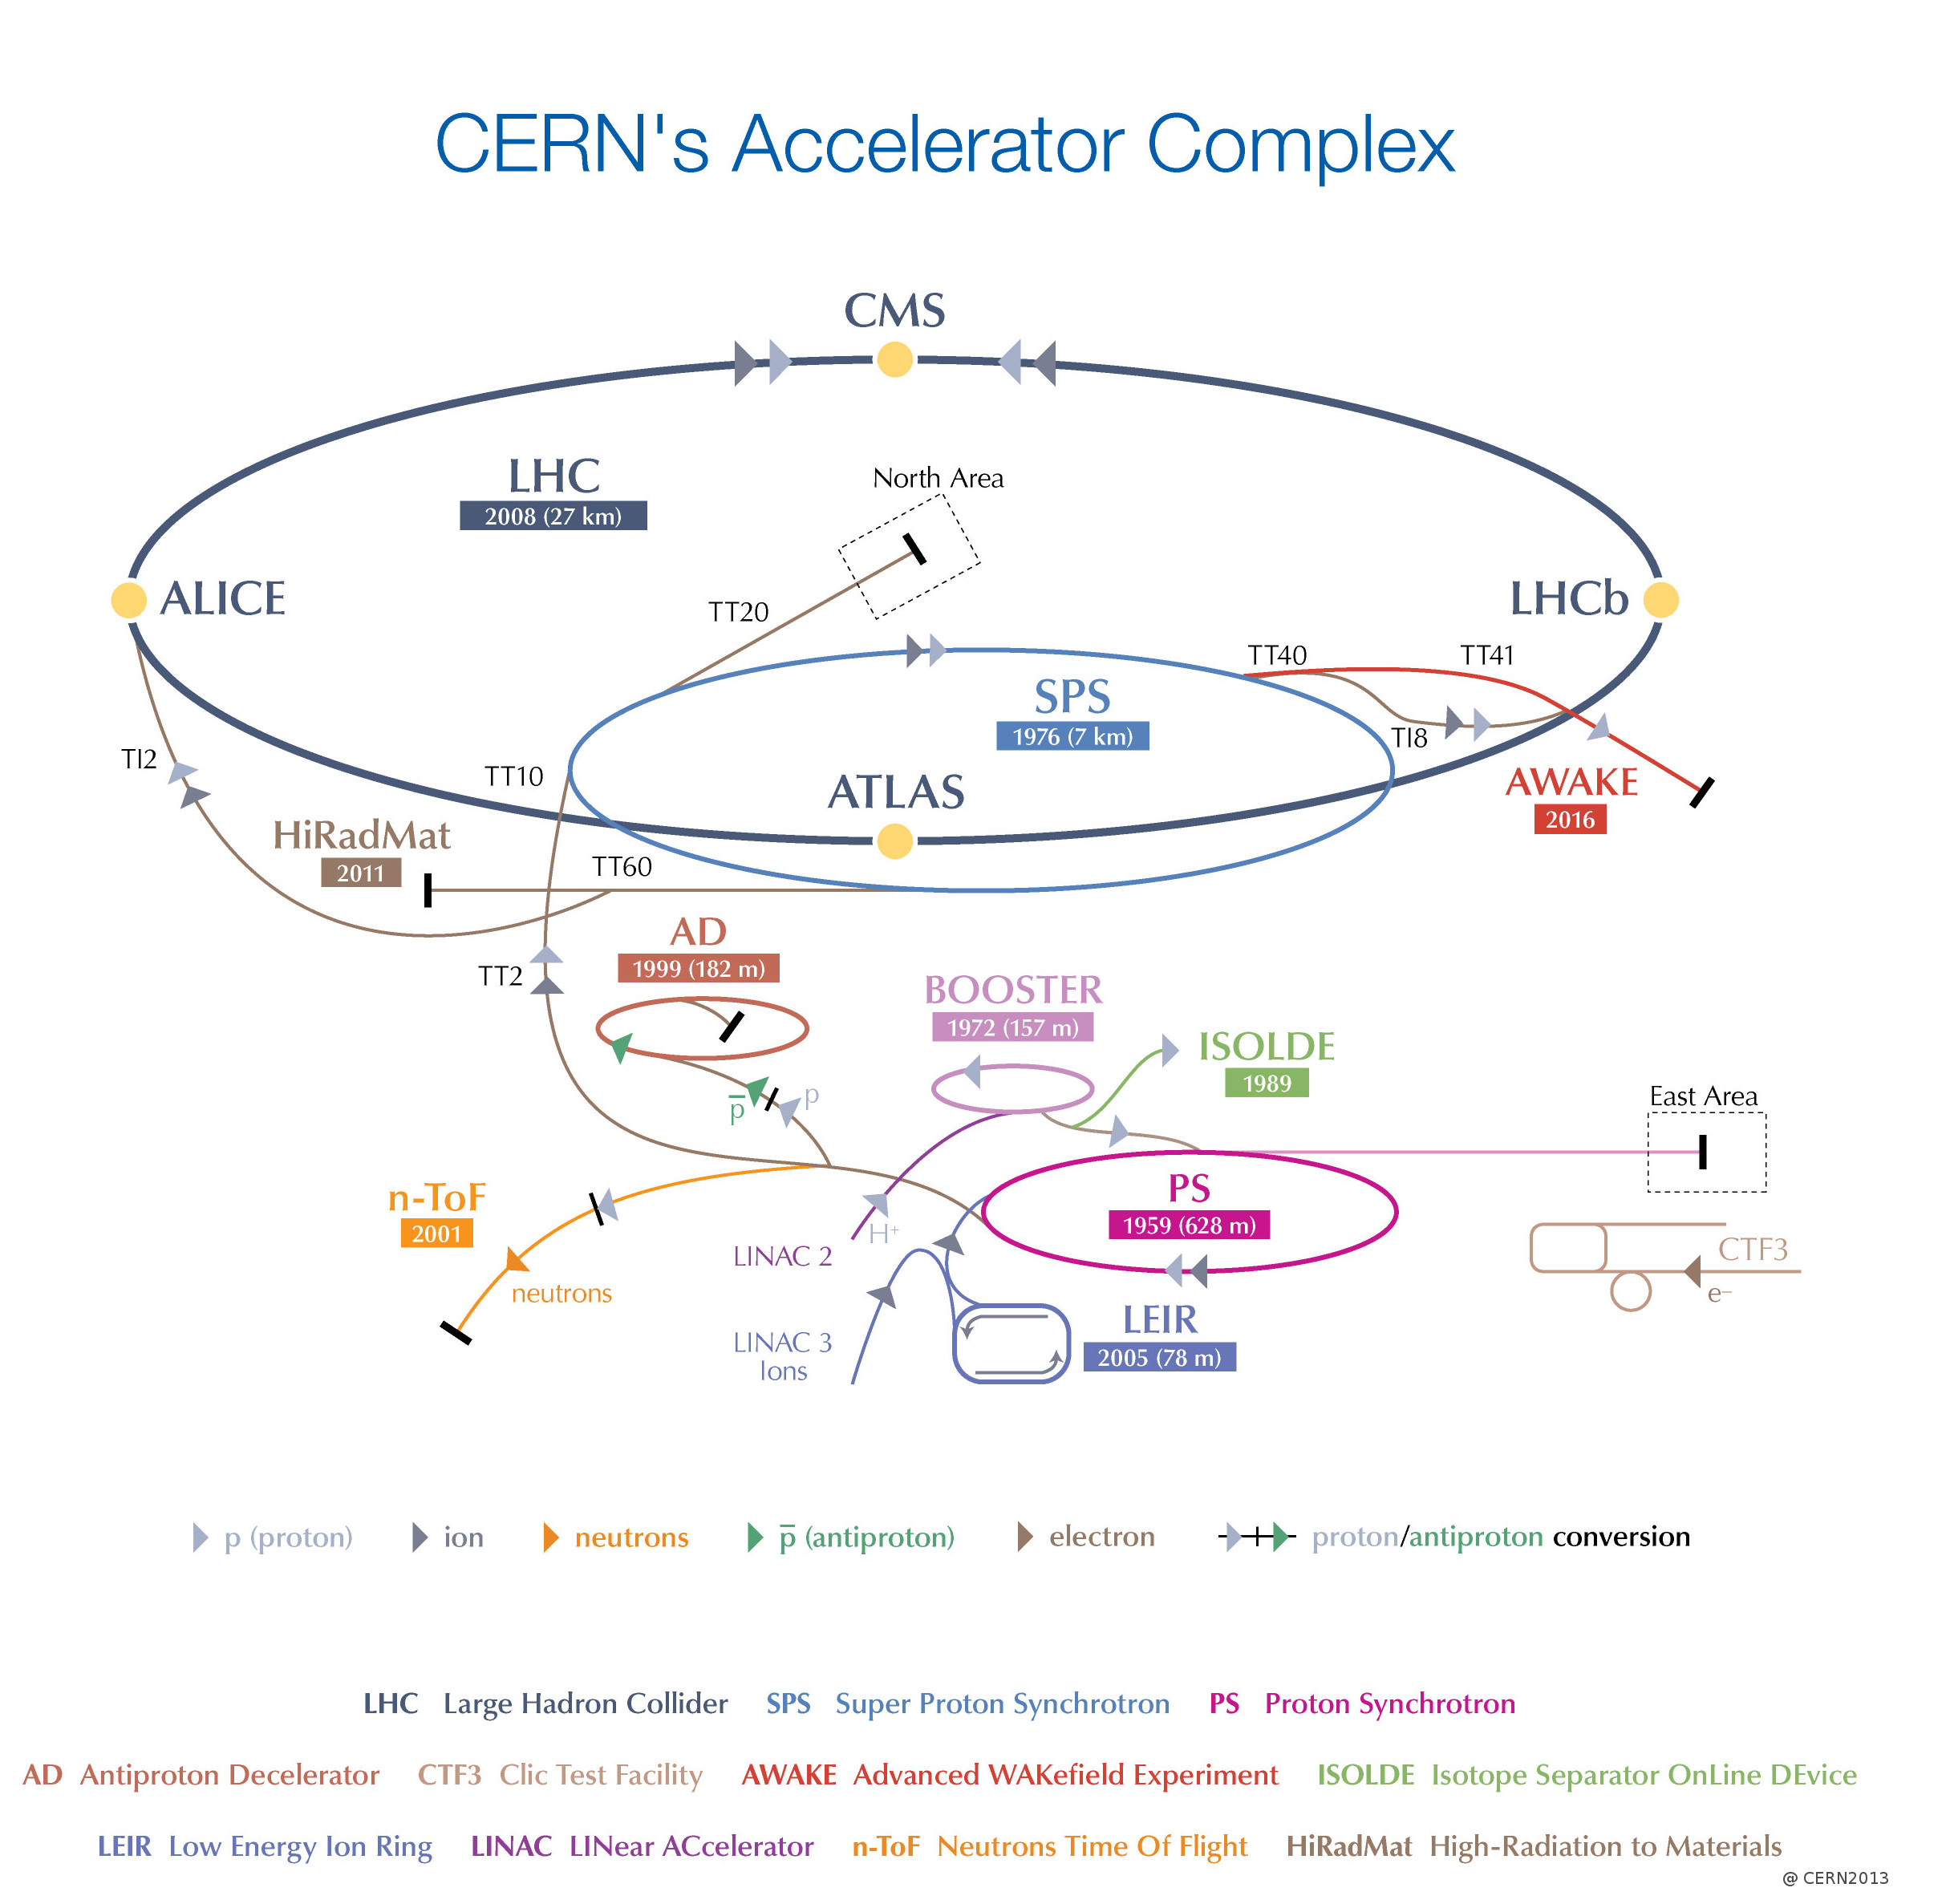
\includegraphics[width=0.98\textwidth]{../figs/Exp/CERN_accelerator_complex2013.jpg}}
    \caption{CERN's accelerator complex. Source of the figure: \cite{ref_fig_CERNacceleratorComplex}.}
    \label{fig:CERN_accelerator_complex}
  \end{center}
\end{figure}

% brochure page 30 (34 of pdf)
\begin{table}[h]
  \begin{center}
  \caption{ Main parameters of LHC \cite{ref_LHC_brochure}}
  \vspace{5 mm}
  \begin{tabular}{|l|c|}
     \hline
     Circumference & 27 km  \\ \hline
     Dipole operating temperature &  1.9 K \\ \hline
     Number of magnets &  9593 \\ \hline
     Number of main dipoles &  1232 \\ \hline
     Number of main quadrupoles &  392 \\ \hline
     Number of RF cavities &  8 per beam \\ \hline
     Nominal energy, protons &  7 TeV \\ \hline
     Nominal energy, lead ions &  2.76 TeV per nucleon \\ \hline
     Peak magnetic dipole field &  8.33 T \\ \hline
     Min. distance between bunches &  7 m \\ \hline
     Design luminosity &  $10^{34}$ cm$^{-2}$ s$^{-1}$ \\ \hline
     No. of bunches per proton beam &  2808 \\ \hline
     No. of protons per bunch (at start) &  $1.1\times 10{11}$ \\ \hline
     No. of collisions per second &  600 millions \\ \hline
  \end{tabular}
  \label{tab:LHCparameters}
  \end{center}
 \end{table}

% begin: LHC lumi and LHC sectors
\begin{figure}
\centering
\begin{minipage}{.48\textwidth}
  \centering
  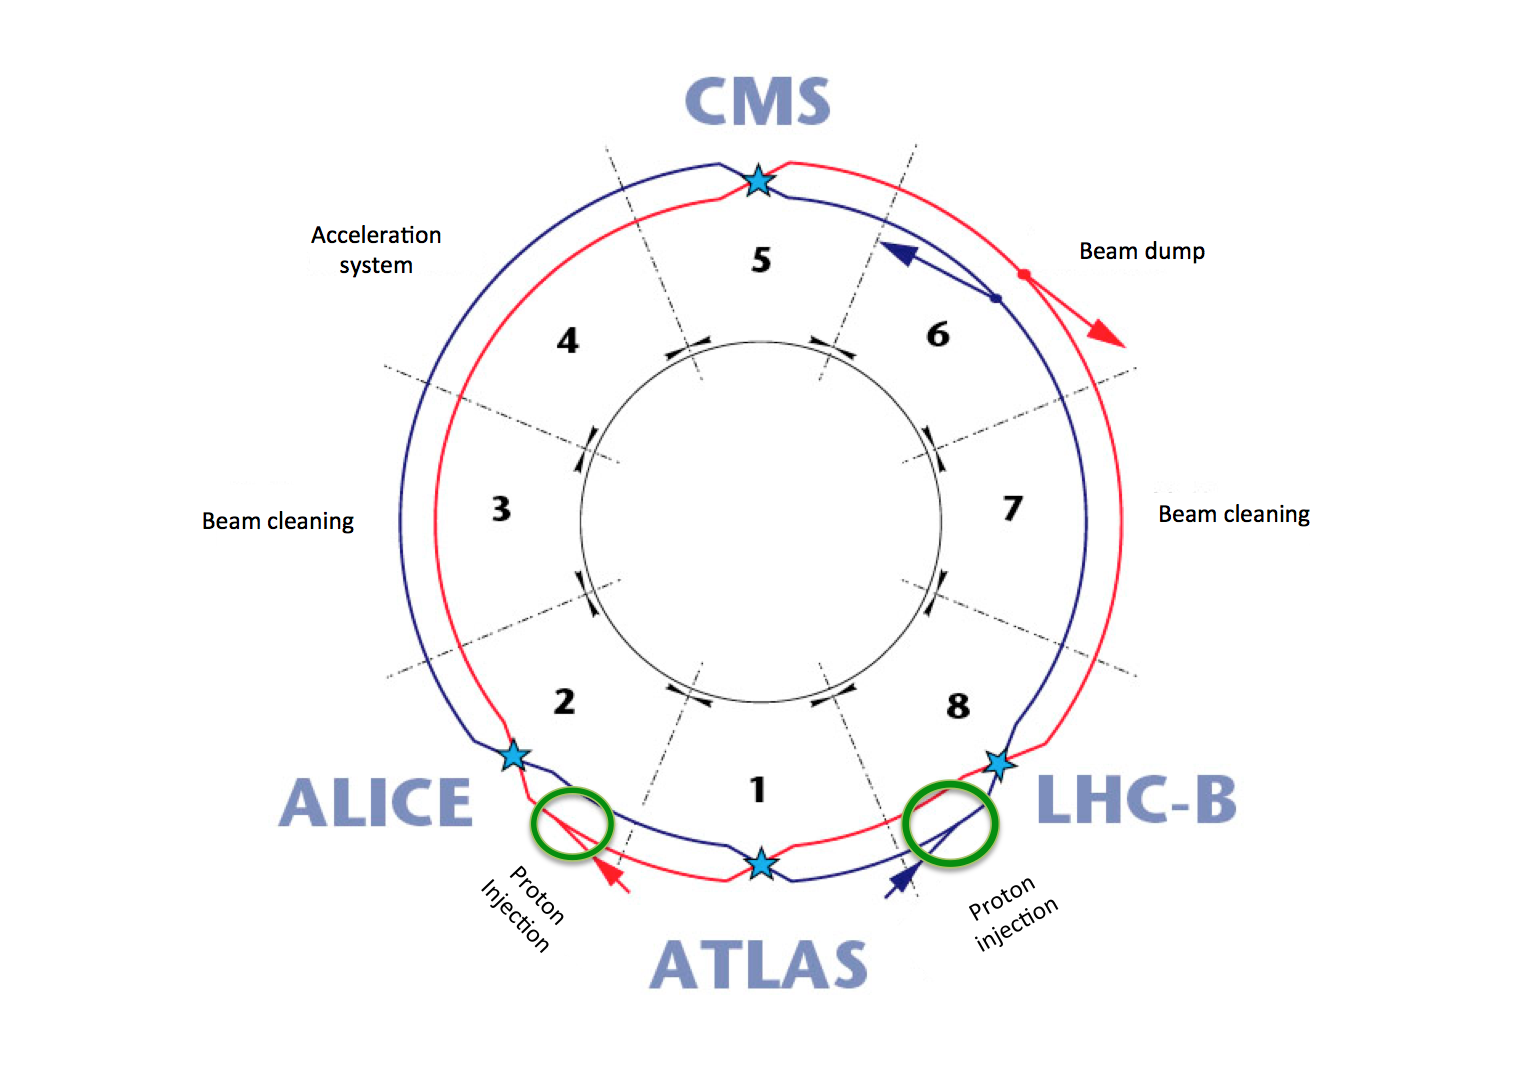
\includegraphics[width=.95\linewidth]{../figs/Exp/LHC_sectors.png}
  \caption{Schematic view of LHC sectors. Source of the figure: \cite{ref_fig_LHCsectors}.}
  \label{fig:LHCsectors}
\end{minipage}%
\begin{minipage}{.48\textwidth}
  \centering
  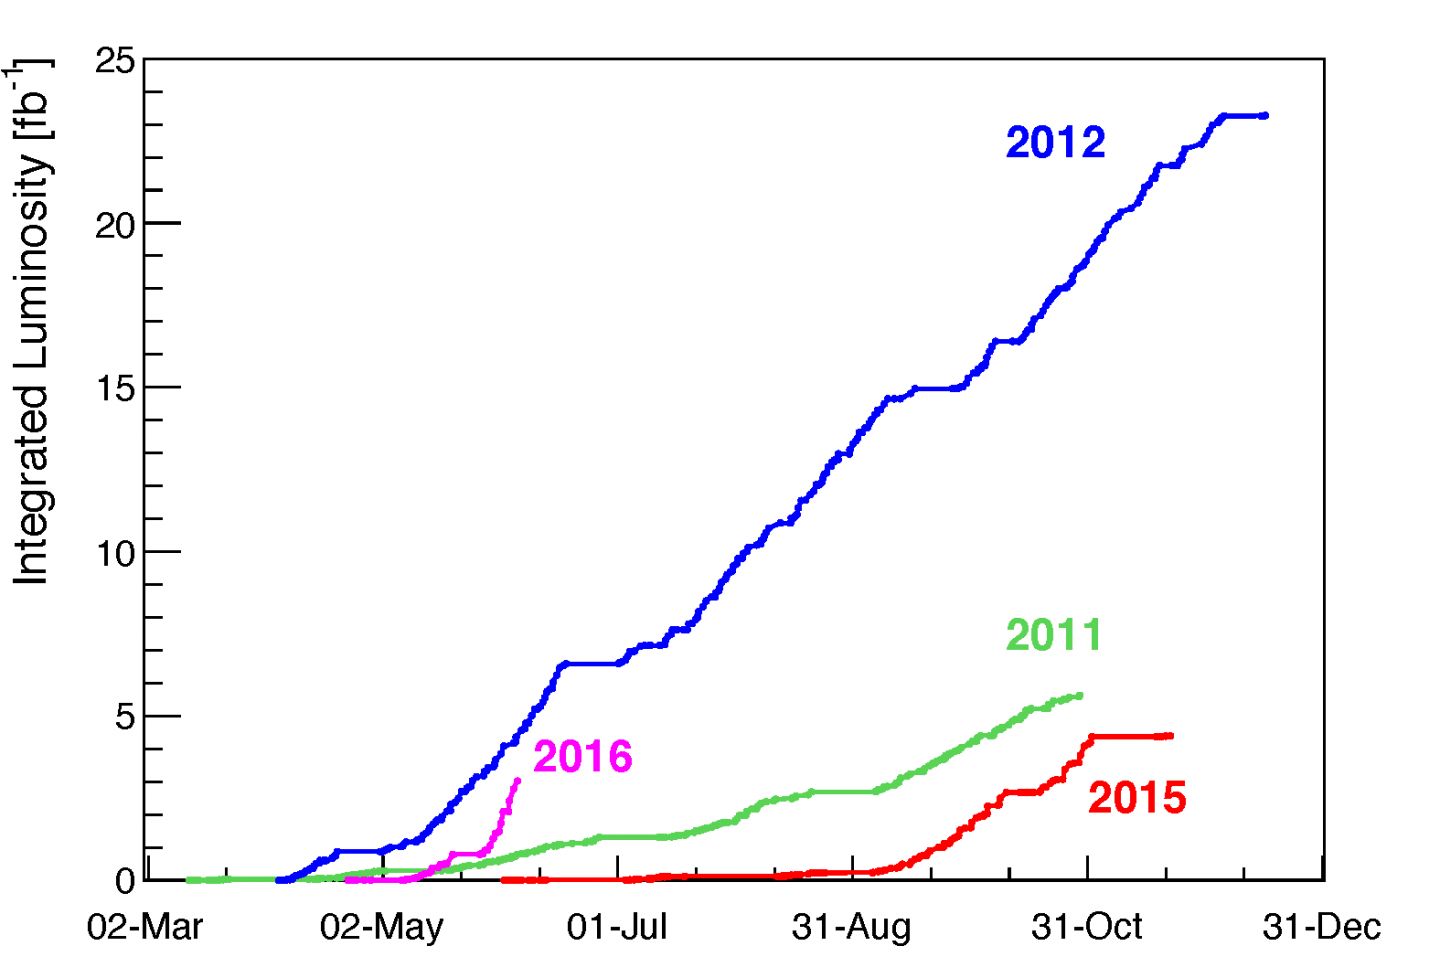
\includegraphics[width=.95\linewidth]{../figs/Exp/LHC_lumi.png}
  \caption{LHC integrated luminosity by year. Source of the figure: \cite{ref_fig_LHClumi}.}
  \label{fig:LHClumi}
\end{minipage}
\end{figure}
% end: LHC lumi and LHC sectors



